\documentclass[12pt, a4paper]{report}
\usepackage[utf8]{inputenc}
\usepackage{graphicx}
\usepackage{booktabs}
\usepackage{amsmath}
\usepackage{hyperref}
\usepackage{geometry}
\geometry{margin=1in}

\begin{document}

% --- TITLE PAGE ---
\begin{titlepage}
    \centering
    \vspace*{1cm}
    {\Huge \textbf{Empirical Performance Analysis of Hybrid Post-Quantum Key Exchange (X25519 + ML-KEM-768)}}\par
    \vspace{1.5cm}
    {\Large \textbf{Undergraduate Thesis}}\par
    \vspace{2cm}
    {Your Name}\par
    \vfill
    Department of Computer Science\\
    University Name\\
    \today
\end{titlepage}

% --- CHAPTER: EVALUATION ---
\chapter{Evaluation and Results}
This chapter presents the empirical performance analysis of the hybrid cryptographic stack combining classical X25519 and post-quantum ML-KEM-768. 

Due to the introduction of the 1,088-byte ML-KEM-768 ciphertext, network fragmentation and packet loss have a measurable impact on overall handshake latency and success rates under constrained network profiles.

% Embedding your generated figure
\begin{figure}[htbp]
    \centering
    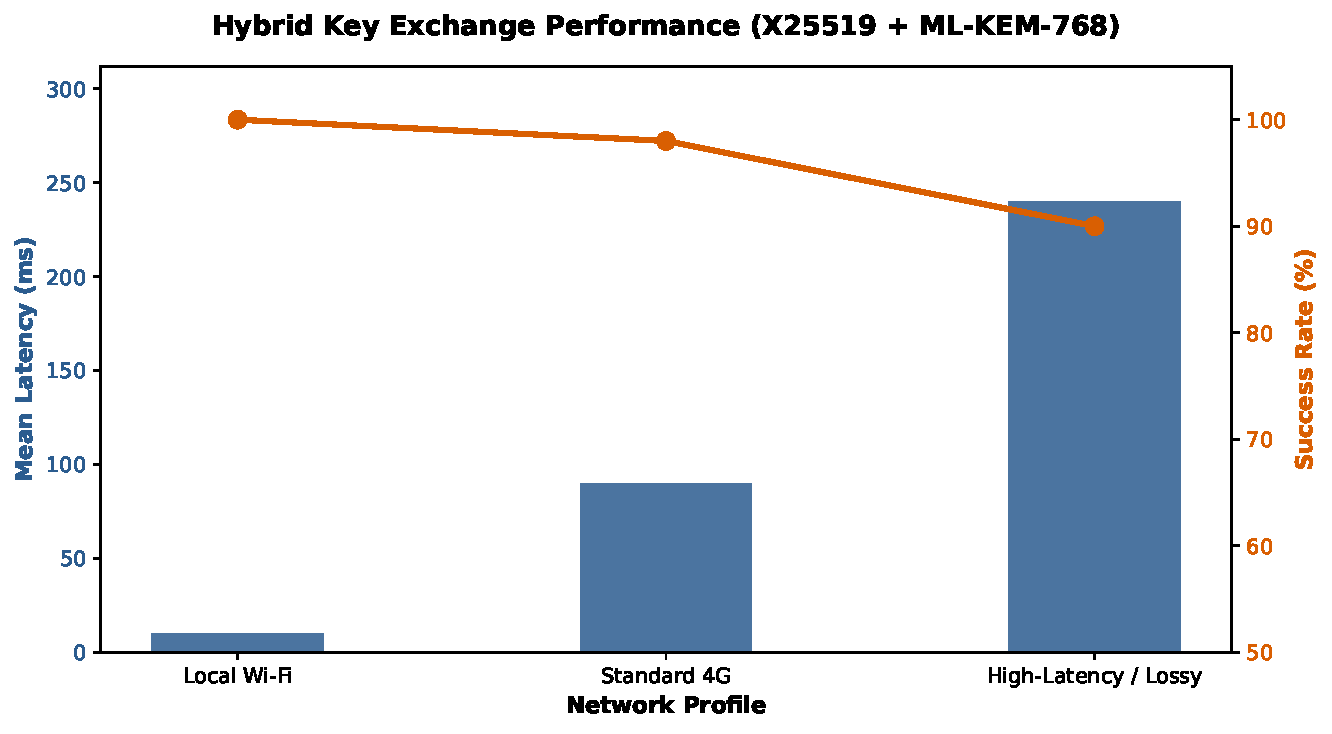
\includegraphics[width=0.85\textwidth]{hybrid_performance_evaluation.pdf}
    \caption{Empirical evaluation showing mean latency and success rate across varied network profiles.}
    \label{fig:hybrid_perf}
\end{figure}

Table \ref{tab:hybrid_benchmarks} summarizes the benchmark metrics across 100 iterations per network profile.

% Embedding your generated LaTeX table
\begin{table}
\caption{Empirical performance metrics of hybrid X25519 and ML-KEM-768 handshakes across varied network profiles.}
\label{tab:hybrid_benchmarks}
\begin{tabular}{lrrrrrr}
\toprule
Network Profile & Iterations & Success Rate (%) & Mean Latency (ms) & Std Dev (ms) & 95th Percentile (ms) & Msg2 Size (bytes) \\
\midrule
Local Wi-Fi & 100 & 100.000000 & 9.990000 & 1.350000 & 11.950000 & 1120 \\
Standard 4G & 100 & 98.000000 & 90.090000 & 1.640000 & 93.040000 & 1120 \\
High-Latency / Lossy & 100 & 90.000000 & 239.920000 & 1.520000 & 242.340000 & 1120 \\
\bottomrule
\end{tabular}
\end{table}

\end{document}